\documentclass[11pt]{article}

\usepackage{cite}
\usepackage{graphicx}
\usepackage[margin=0.88in]{geometry}
\usepackage[font=small,labelfont=bf]{caption}

\begin{document}

\begin{center}
    \huge
    \textbf{Spiral Packing}
    
    \vspace{0.1cm}
    \Large
    \textbf{Adrian Cortez}
    
    \vspace{0.1cm}
    \small
    \textbf{Rochester Institute of Technology}
    \vspace{0.3cm}
\end{center}

	The paper "Spiral Packing" by Cameron Browne and Paul van Wamelen \cite{Browne2006834} presents an iterative method for generating artistic space-filling designs based on spiral packing. Figure~\ref{fig:example} shows example images generated using the spiral packing algorithm. The goal of this project is to implement and evaluate the algorithm described in the paper. The project advisor is Dr. Roger Gaborski.
	
\begin{figure}[ht]
	\centering
	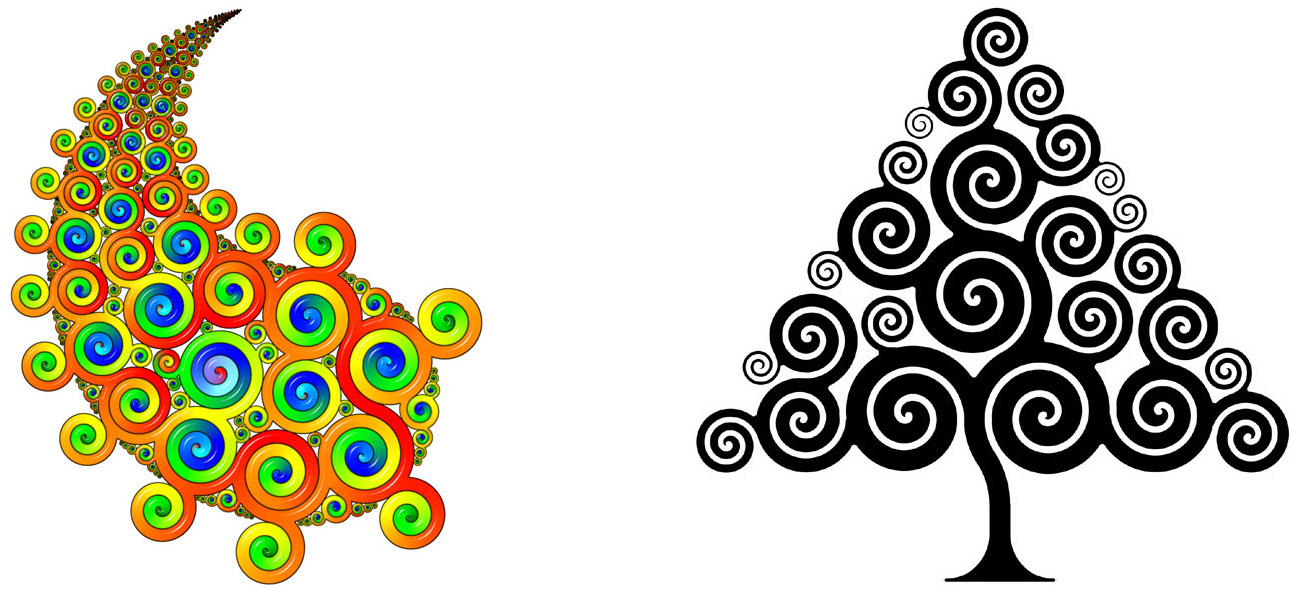
\includegraphics[width=90mm,height=40mm]{spiral-packing-example}
	\caption{Examples of spiral packing. \cite{Browne2006834}}
	\label{fig:example}
\end{figure}

	Spiral packing is the process of filling a given area, or shape boundary, to a desired level with connected sets of spirals. The connected sets are generated by branching child spirals from parent spirals, adhering to the following constraints: A child spiral (1) may have at most one parent; (2) must not have a greater width than its parent; (3) must meet its parent tangentially; (4) must be rotated such that its terminal point lies on the line drawn between its center and its parent's center; and (5) may touch neighboring spirals tangentially but may not intersect them. 
	
	The general polar equation for the Archimedean spiral is \begin{math}r = a\theta^\frac{1}{n}\end{math}. The proposed algorithm utilizes the special case of the Archimedean spiral (\begin{math}n=1\end{math}), known as Archimedes' spiral, described by the equation \begin{math}r = a\theta\end{math}. This special case was chosen by the authors because of its aesthetic and well-behaved mathematical qualities. The Archimedes' spiral can be described in cartesian coordinates by the set of parameters \begin{math}(x,y,w,\theta,T,\omega)\end{math}, giving the equations:
	\begin{equation}x_{s}(t) = x + wt cos(\theta + 2\pi\omega t)\end{equation}
	\begin{equation}y_{s}(t) = y + wt sin(\theta + 2\pi\omega t)\end{equation}
for \begin{math}0 \leq t \leq T\end{math}, where \begin{math}(x,y)\end{math} is the spiral's center, \begin{math}w\end{math} is the width of one rotation, \begin{math}\theta\end{math} is the starting angle or phase, \begin{math}T\end{math} is the number of rotations or total sweep of the spiral, and \begin{math}\omega\end{math} is the orientation of the spiral (\begin{math}\omega = -1\end{math} for clockwise and \begin{math}\omega = 1\end{math} for counterclockwise).

	There are three general geometric cases to consider when generating connected spiral sets. The first, and most simple, of these cases is the branching of a child spiral that does not intersect any neighboring spirals, as shown in Figure~\ref{fig:geo}a. This is handled simply by drawing the child spiral at the preferred location. The other two cases occur when the child spiral intersects one or two neighboring spirals  when attempting to place the child in the preferred location, shown in Figure~\ref{fig:geo}b and c respectively. In both cases, the child spiral may need to be resized or repositioned, within a threshold, so that it can lie tangent to the neighboring spirals. In the case of two neighboring spirals being intersected, the algorithm may not converge in a way to allow the child spiral to lie tangent to both neighbors. In this case, the maximally intersected neighbor is chosen as the spiral to position the child spiral tangent to.

\begin{figure}[ht]
	\centering
	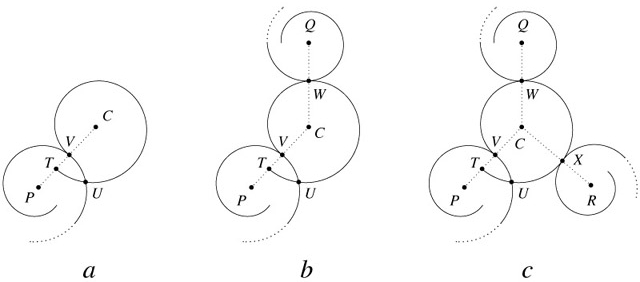
\includegraphics[width=100mm,height=40mm]{spiral-packing-fig-01}
	\caption{The three geometric cases when branching: (a) simple branching, (b) fitting the child spiral to one neighboring spiral, and (c) fitting the child spiral to two neighboring spirals. \cite{Browne2006834}}
	\label{fig:geo}
\end{figure}

	To simplify the process of fitting a child spiral to neighboring spirals, the spirals are approximated using circles. This essentially reduces the spiral packing problem to the circle packing problem, also known as Apollonian packing. This simplification makes it easier to determine when child spirals intersect neighboring spirals and solving the circle packing problem for the circle of minimum radius provides a good approximation for the placement and size of the fitted child spiral.

	To begin the generation of the connected spiral sets, the implemented program will use a pair of seed spirals from which the child spirals can branch. During the branching process, the user will need to provide a preferred location for the child spirals. The algorithm will take this preferred location in conjunction with the constraints listed above and the state of the packed area to attempt to place the child spiral. The goal is to place the child spiral as close to the user's preferred location as possible without violating the constraints.

	The results of the algorithm will be evaluated in two ways. The first evaluation technique is purely visual; the algorithm must produce images that are aesthetically pleasing as well as space-filling. This is determined not only by the generated connected spiral sets adhering to the constraints listed above, but also by the coloring of the resulting images. In order to properly evaluate the robustness of the implementation, several images will be generated to demonstrate different packing scenarios, bounding areas, arrangements, and color schemes. The second way of evaluating the results is by calculating the \textit{porosity}, or the ratio of vacant area to the area covered by spirals. The lower the porosity, the better the packing. For the purposes of this project, a porosity of 5\% or lower will be considered a good packing. 
	
	The project will be completed over the course of twelve weeks, divided into three milestones. The work done over the twelve weeks will culminate into an implementation of the proposed spiral packing algorithm and a final report. The first milestone includes the outline of the final paper and a description, in pseudocode, of the algorithm to implement. This milestone also includes a program capable of drawing Archimedean spirals given the set of parameters mentioned previously. The second milestone will deliver completed drafts of the introduction, background and related works sections of the final paper. Also included is an implementation of spiral branching to generate the connected spiral sets, handling all three cases described previously. Preliminary results and examples of generated images are also delivered during this milestone. The final milestone delivers the completed final paper and completed implementation. This includes spiral packing within an arbitrary boundary and the addition of generated color. Both flat and gradient color will be implemented to provide a better visual aesthetic.

	The final paper will be a minimum of 7 pages the in ACM SIG Proceedings format. Included in the final paper will be several generated images (not included in the page count) demonstrating the spiral packing algorithm applied to different packing scenarios and bounding areas.
	
\begingroup
\renewcommand{\section}[2]{}%
\bibliographystyle{plain}
\bibliography{references}{}
\endgroup

\end{document}